\documentclass{article}
\usepackage[utf8]{inputenc}
\usepackage{amsmath}
\usepackage{float}
\usepackage{graphicx}
\usepackage{multicol}
\usepackage{nips15submit_e,times}
\usepackage{hyperref}
\usepackage{url}
\usepackage{amssymb}

\title{Similar Language Detection}
\author{Shenglan Qiao \\
Stanford University\\
%Stanford, CA 93405 \\
%\texttt{shenglan@stanford.edu} \\
\And
Daniel L\'{e}vy \\
Stanford University\\
%Stanford, CA 93405 \\
%\texttt{danilevy@stanford.edu} \\
}
\date{November 2015}

\newcommand{\fix}{\marginpar{FIX}}
\newcommand{\new}{\marginpar{NEW}}

\nipsfinalcopy % Uncomment for camera-ready version

\begin{document}

\vspace{-2cm}

\maketitle

\begin{abstract}
Language identification is a key component of multiple NLP applications. Discriminating between similar languages is one of the bottlenecks of state-of-the-art language identification systems. In this paper, we present a hierarchical method that first classifies a written sentence into a linguistically defined language group and then determines the language. We are able to achieve an overall test accuracy of $92.6\%$ (12039/13000). Our method is robust and easily scalable to incorporate many languages as well as more training data.
\end{abstract}

%\begin{multicols}{1}

\section{Introduction}

Language identification has many applications across different domains (translation, language interpretation, etc.). While it is trivial to discriminate between disparate languages, it is far from a solved one for highly similar languages and dialects. Our problem is presented in the Discriminating Similar Language (DSL) Task, a contest that requires teams to predict the language of sentences written in similar languages. The categories can be different languages or variations of the same languages; distinguishing one from another is far from trivial. For example, in the training dataset provided by DSL, more than $20\%$ of the sentences in the South-West Slavic group were written with words present in all three languages, making it impossible to solve with a simple dictionary look-up.

In this paper, we present a hierarchical method that breaks down the problem into two consecutive stages. Languages are grouped by their degrees of similarity into groups. A simple word-frequency method first identifies the group a written text belongs to. A more sophisticated method using an ensemble of Support Vector Machine (SVM) classifiers then determines the language within the group.We have also developed this method with efficiency and scalability in mind. Our computing resources were limited to our personal computers; we had to find a way to keep the size of the data and the complexity manageable without sacrificing too much accuracy.

\section{Related Work}

Classifying tests written in disparate languages is considered a solved problem. \cite{MacNee} presented the word frequency method for language classification, which we used for discriminating among language groups. 

Discriminating among similar languages is a fairly present subject in literature and still open for discussion. In September 2015, the LT4VarDial, a joint workshop on Language Technology for closely related language, varieties and dialects was held in Bulgaria. This workshop featured the DSL Task, a contest where teams were given a training set to build models that would be tested on an undisclosed testing set. This shared task inspired several research papers on the subject (an overview can be seen in \cite{dsl-overview}).

\cite{dsl-winner} introduced us to the idea of an ensemble classifier. However, \cite{dsl-winner} included all languages in a single ensemble classifier. We decided this method would be difficult to scale up to include more languages to multiple languages; it would also be computationally inefficient or impossible for us given our limited resources. \cite{two-steps} convinced us that a hierarchical methods could perform almost as well as the winner of the task while being more robust and scalable.

\section{Dataset and features}

The data sets we used were part of the DSL-Shared Task of 2015. The task provided participants with training (17000 examples per language), development (2000 examples per language) and testing sets (1000 examples per languages). The sets consisted of individually labeled sentences extracted from the journalistic corpora in 13 different languages. The languages were part of 6 language groups.
\begin{itemize}
\item South-Eastern Slavic (ses): Bulgarian (bg), Macedonian (mk)
\item South-Western Slavic (sws): Bosnian (bs), Croatian (hr), Serbian (sr)
\item West Slavic (ws): Czech (cz), Slovak (sk)
\item Spanish(es): Argentine Spanish (esar), Peninsular Spanish (eses)
\item Portuguese (pt): Brazilian Portuguese (ptbr), European Portuguese (ptpt)
\item Austronesian (aus): Indonesian (id), Malay (my)
\end{itemize}

We engineered two categories of features (word and character) and we represented them in a sparse way: \textbf{word $n$-grams} (for example, given a sentence $w_1 \ldots w_n$, the $2$-grams are $w_1w_2, w_2w_3, \ldots, w_{n-1}w_n$) and \textbf{character $n$-grams}: the same than above but with characters instead of words (with character cross-over between words). For example, the 5-grams of "Hello World" are "Hello","ello ","llo W", "lo Wo", "o Wor", " Worl", "World". 


We used words $n$-grams for $n\in\{1,2\}$ and character $n$-grams for $n \in \{3, \ldots, 6\}$.

\section{Methods}
The hierarchical method employs a simple word-frequency method that first identifies the group a test belongs to. It then uses an ensemble of SVM models to determine the final output. Figure~\ref{fig:schema} shows a schematic representation of the method. The SVM models are trained with examples within the language group and can have different number and combination of features across groups.

\begin{figure}[h!]
\centering
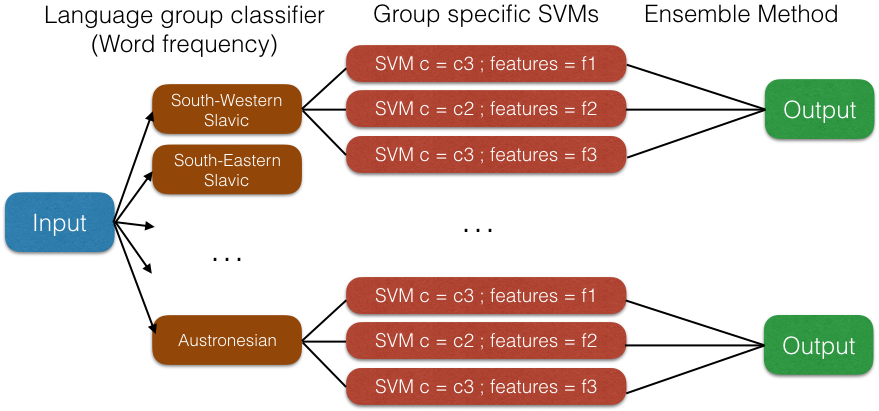
\includegraphics[scale=0.33]{schema.jpeg}
\caption{Overview of our learning algorithm.}
\label{fig:schema}
\end{figure}

In this section, we will describe the two stages of our hierarchical method as well as our protocol to avoid over-fitting. Parameters of our method were tested and tuned with the development dataset, before applying it to the test dataset. 

\subsection{The Word-Frequency method}

The first block of our pipeline is a classifier to distinguish the language group of an input. We built this classifier using the following word-frequency method. From the training set, for each language $l \in 1\ldots 13$, we define $x^l \in \mathbb{R}^{1000}$ s.t. $x_i^l$ is the frequency of the $i$th common word of the $l$th language.

Given an unclassified sentence $s$, we define $x^l(s), l=1\ldots 13$ s.t. $x_i^l(s) = 1$ if the $i$th word of the $l$th language is present in the sentence. The classifier is then $h(s) := \underset{l\in 1 \ldots 13}{\mathrm{argmax}} \langle x^l(s), x^l \rangle$. To obtain the group, we then just have to return the group the language $h(s)$ is part of.

McNamee showed in \cite{MacNee} that this word frequency method was extremely effective when it came to classifying rather distinct languages. This method also proved computationally efficient and obtained virtually perfect result ($>99\%$ accuracy) for differentiating among language groups, which we will go more in-depth into in section \ref{discussion}.

\subsection{Multi-class SVMs}

In class, we derived the optimization program for $2$-class SVM. In \cite{multiclass}, Crammer and Singer makes a derivation for a multi-class SVM which we are using.

Let's replace ourselves in the context of the course but with $k$ classes this time. 

Let $(x^{(i)}, y^{(i)}), i=1\ldots m$ with $x^{(i)} \in \mathbb{R}^n$ but $y^{(i)} \in \{1 \ldots k\}$. Crammer and Singer (2002) proposed the following multi-class approach by solving the following optimization problem:

\begin{equation*}
\begin{aligned}
& \underset{w_l, \xi_i, l=1\ldots k, i = 1\ldots m}{\text{minimize}}
& & \frac{1}{2} \sum\limits_{l=1}^k w_l^Tw_l + C \sum\limits_{i=1}^m \xi_i\\
& \text{subject to}
& & w_{y_{(i)}}^Tx^{(i)} - w_l^Tx^{(i)} \leq \delta_{i,l} - \xi_i, \; i = 1, \ldots, m.
\end{aligned}
\end{equation*}

Where $\delta_{i,l} = 1$ if $i=l$, $\delta_{i,l} = 0$ if $i \neq l$.

With the following decision function: $$h_{w_1, \ldots, w_k}(x) = \underset{l\in\{1,\ldots,k\}}{\mathrm{argmax}} w_l^Tx$$

We can derive the dual problem:
\begin{equation*}
\begin{aligned}
& \underset{\alpha_i^l, l=1\ldots k, i = 1\ldots m}{\text{minimize}}
& & \sum\limits_{1\leq i,j \leq m, 1\leq l \leq k} \alpha_i^l \alpha_j^l \langle x^{(i)}, x^{(j)}\rangle + \sum\limits_{1\leq i \leq m, 1\leq l \leq k} \delta_{i,l} \alpha_i^l\\
& \text{subject to}
& & \sum\limits_{l=1}^k \alpha_i^l, \; i = 1, \ldots, m. \\
& & & \alpha_i^l \leq \delta_{i,l}C, \forall i \in \{1, \ldots, m\}, \forall l \in \{1, \ldots k \}
\end{aligned}
\end{equation*}

Where $w_l = \sum\limits_{i=1}^m \alpha_i^l x^{(i)}, l=1\ldots k$

We can then solve the dual using the coordinate ascent method seen in class. It is clear that this extension from $2$ classes to $k$ classes works in the exact same way than before and that this classifier has the same properties (kernel trick...). We used LIBLINEAR SVM to implement this multi-class SVM.

\subsection{Feature scoring using tf-idf}

Character $n$-grams for higher values ($n\geq 4$ mostly) are very prone to over-fitting. In order to make our method robust, we had to select a subset of features for the ensemble of SVM models. Due to the size of our features set (approximately $3$ millions) both PCA and forward/backward search were out of the question. To overcome this obstacle, we decided to score the features using tf-idf and use only the top-rankings ones.

We defined the tf-idf score of a feature $t$ derived from training set $D$ to be
\begin{equation}
\mathrm{tfidf}(t,D) = \mathrm{tf}(t,D) \times \log \frac{N}{\mathrm{df}(t,D)}
\end{equation}
where $\mathrm{tf}(t,D)$ is the total number of times $t$ appeared in the training set, $\mathrm{df}(t,D)$ the number of examples that contain $t$, and ${N}$  the number of training examples. Since $N/df(t,D)$ if always greater or equal to 1, this definition of tf-idf is always non-negative. It is zero if the feature appears in every training example; intuitively, this means the feature is common to all languages in the training set and therefore cannot help distinguish them from one another.

\subsection{Ensemble methods}

To reduce variance, we also decided to train several SVM models on a given language group and combine them using ensemble methods. For each language groups, we trained $p$ SVM using different hyper-parameters (features and $C$ constant). Each one of these SVM $i$, outputs $k$ weight vectors. We have $\left(w_{i,l}\right)_{1\leq i \leq p, 1 \leq l \leq k}$ weight vectors at our disposition.

After experimenting with several ensemble methods (majority vote, boosting, and mean confidence) we settled on mean confidence, which can be written as follows:

$$h_{\left(w_{i,l}\right)_{1\leq i \leq p, 1 \leq l \leq k}}(x) = \underset{1\leq l \leq k}{\mathrm{\arg \max}} \langle \sum\limits_{t=1}^p w_{t,l}, x\rangle$$

For some language group, we did not need to use the ensemble method as high-accuracy classification was straightforward. For the others, we trained and combined 5 SVMs, each had a combination word 1-grams, 2-grams, and character n-grams ($n \in \{3,4,5,6\}$).

\section{Results and Discussions}\label{discussion}
Our final classification results for the test set are shown in figure~\ref{fig:ConfMat}. Our hierarchical method yields an overall accuracy of $92.6\%$ (12039/13000). For $99.5\%$ of the test examples, the word-frequency method assigns them correctly to their respective language group. We chose to combine the South-Western and West Slavic languages into one group (the sws-ws group) since the word-frequency method tended to group these five languages together. 
\begin{figure}[h!]
\centering
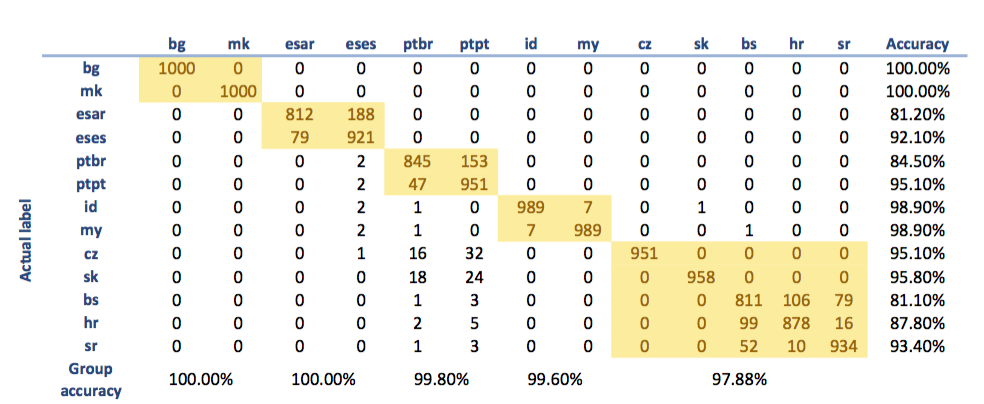
\includegraphics[scale = 0.4]{Final_confusion_matrix.png}
\caption{Confusion matrix for all 13 languages. Group accuracy means the rate at which the word-frequency method correctly identified the language group of test examples.}
\label{fig:ConfMat}
\end{figure}

In order to avoid over-fitting, we tuned the regularization parameter $c$ and performed feature selection based on tf-idf scoring. Within each language group, multiple SVM models were built and tested on the development set. Test accuracies of these model as a function of $c$ were plotted. For each SVM model, we chose the value for $c$ at which the testing accuracy gain was marginal compared to the training accuracy gain.

%\begin{figure}[h!]
%\centering
%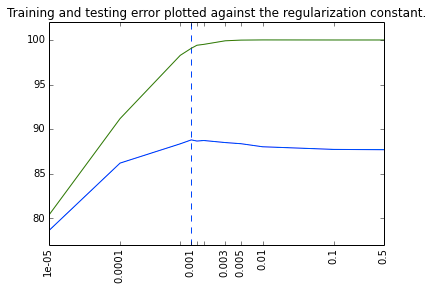
\includegraphics[scale = 0.45]{regularization_constant.png}
%\caption{Training and testing accuracy on the development set (sws-ws language group) as a function of the regularization parameter $c$.}
%\label{fig:RegConst}
%\end{figure}

We selected subsets of features for our final SVM models by observing how their prediction accuracies on the development set changed as a function of features. We ranked features by category (word 1-grams, 2-grams and character n-grams, $n \in \{3,4,5,6\}$) using the tf-idf scores defined in the method section. Starting with the highest ranking features, we computed test accuracies on the development set using model trained with increasing number of features. Figure~\ref{fig:TopFeatures} shows an example of plots we used for feature selection in the sws-ws group. Similar to tuning $c$, our feature selection protocol kept the top-ranking $n$ features in our final SVM or ensembles (in figure~\ref{fig:TopFeatures} n = 30000) by which increasing the number of features stopped gaining any significant test accuracy on the development set. 

\begin{figure}[h!]
\centering
\begin{minipage}{0.45\textwidth}
\centering
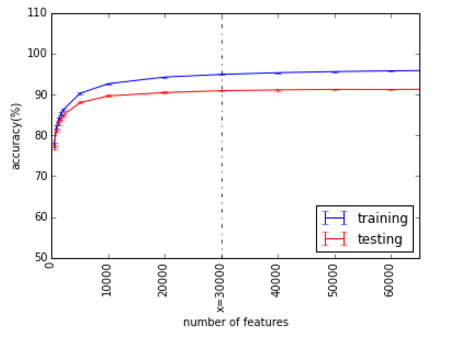
\includegraphics[scale = 0.45]{num_features_vs_accuracy.png}
\caption{Prediction accuracy on the development set (sws-ws language group)  as a function of the number of top-ranking features.}
\label{fig:TopFeatures}
\end{minipage}
\hfill
\begin{minipage}{0.45\textwidth}
\centering
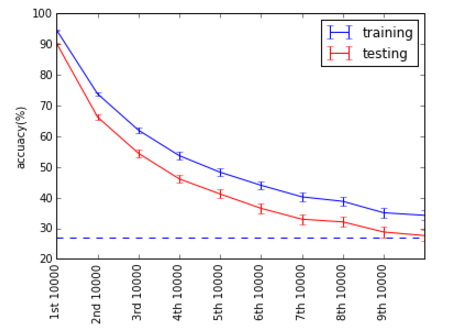
\includegraphics[scale = 0.45]{accuracy_vs_feature_sets.png}
\caption{Prediction accuracy on the development (sws-ws language group)  set as a function of sets of increasingly lower-ranked SVM features.}
\label{fig:FeatureSets}
\end{minipage}


\end{figure}

Finally, we also demonstrated that the definition of tf-idf was appropriate for feature selection. SVMs built with lower ranking features had lower test accuracies when applied to the development set. For instance, figure~\ref{fig:FeatureSets} shows that test accuracy of models built with sets of word 1-grams decreased monotonically; the first set contained the 10000 top-ranking features, and the successive sets contained the same number of increasingly lower-ranked features. This consistent trend proved that we were avoiding over-fitting by retaining features most representative of the training data.

\section{Conclusion}
We have achieved classification of 13 similar languages with an overall accuracy of $92.6\%$. This is close to the DSL Task winning team's accuracy of $95\%$. More importantly, we have explored a method that is easily scalable and robust. The word-frequency classifier requires maintaining a database of only one thousand frequently occurring words per language. SVM features are derived within a language group, typically made up of only two languages. Generalizing to many languages therefore does not require changing the modeling for existing languages in the hierarchical model but simply adds independent branches to the hierarchy. This advantage of scalability stems from the linguistic knowledge used to divide languages into groups. Additionally, our methodical selection of features and the regularization parameter has rendered our method robustness across the development and test sets. This gives us confidence that given more training data our method will perform well on a variety of texts.

Future work will involve improving performance on certain language groups. Our method prefers to label the test examples as a certain language within the South-Western Slavic, Spanish, and Portuguese groups. More investigation is needed to explain why this happens. Gathering training data from genres other than journalistic articles can also be valuable and may improve the performance of our method. 


\newpage

\bibliographystyle{amsplain}
\begin{thebibliography}{10}

\bibitem{MacNee} McNamee, P.,2005
\textit{Language identification: a solved problem suitable for undergraduate instruction}. Journal of Computing Sciences in Colleges, 20(3):94–101.

\bibitem{Franco-Sal} Franco-Salvador, M., Rangel,F.,Rosso,P.,Taule,Marti,M.,A.,2015.\textit{Language variety identification using distributed representations of words and documents}. Proceeding of the 6th International Conference of CLEF on Experimental IR meets Multilinguality, Multimodality, and Interaction (CLEF 2015), volume LNCS(9283). Springer-Verlag.

\bibitem{dsl-overview} Zampieri, M., Tan, L., Ljubesic, N., Tiedemann, J., Nakov, P., \textit{Overview of the DSL Shared Task 2015}. Proceeding of the LT4VarDial Workshop.

\bibitem{dsl-winner} Malmasi, S., Dras, M., \textit{Language Identification using Classifier Ensembles}. Proceeding of the LT4VarDial Workshop.

\bibitem{dsl-other} Franco-Salvador, M., Rosso, P., \& Rangel, F. 2015., \textit{Distributed Representations of Words and Documents for Discriminating Similar Languages}. Proceeding of the LT4VarDial Workshop

\bibitem{two-steps} Acs, J., Grad-Gyenge L., Bruno Rodrigues de Rezende Oliveira, T. 2015. \textit{A two-level classifier for discriminating similar languages}. Proceeding of the LT4VarDial Workshop

\bibitem{multiclass} Crammer, K., Singer, Y. 2002 \textit{On the Learnability and Design of Output Codes for Multiclass Problems}. Machine Learning, Vol. 47.

\end{thebibliography}
%\end{multicols}
\end{document}
